% Muc 4.3 (moi, tach tu muc 4.2)  --  phu trach: Hùng
% nguon: python/quant/pipeline_int.py (cua so, z-score, RR so nguyen); docs/system_overview.md §7 (tang 6-8);
%        trung vi dac trung RR: cache beats_annotation cua repo 1DCNN, 22 ban ghi DS1
\section{Trích xuất đặc trưng}\label{sec:dactrung}

Từ tín hiệu đã lọc $y$ và vị trí đỉnh R của khối tiền xử lý, khối trích xuất đặc trưng tạo ra hai đầu vào của mạng cho mỗi nhịp: cửa sổ $z_q$ gồm 360 giá trị int8 mô tả hình dạng nhịp và bốn đặc trưng $\mathrm{rr}_q$ mô tả nhịp điệu.
Hình~\ref{fig:ch4-khoidactrung} trình bày hai nhánh của khối.

\begin{figure}[htbp]
  \centering
  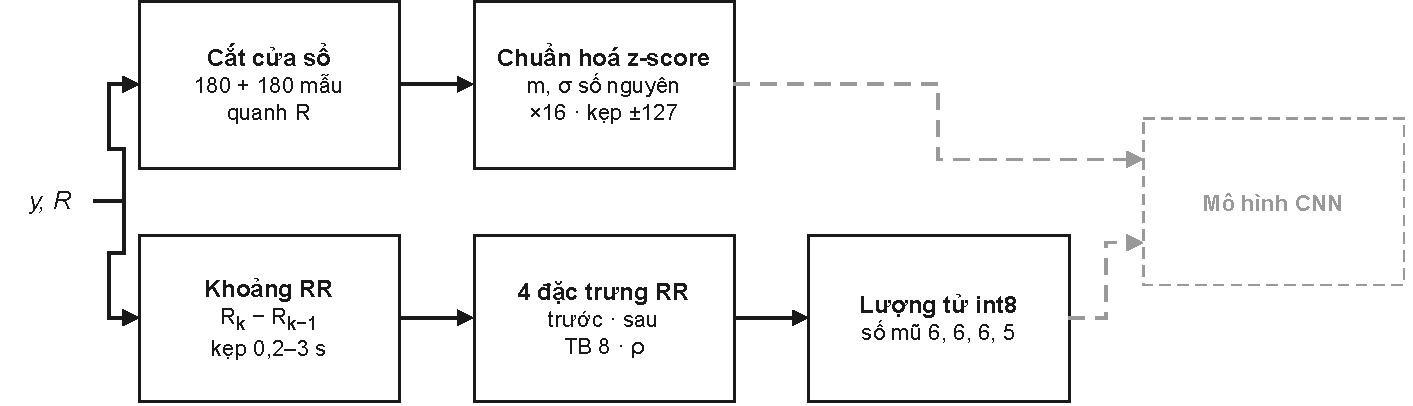
\includegraphics[width=\textwidth]{ch04_mo_hinh_cnn/khoi_dactrung}
  \caption{Các khâu của khối trích xuất đặc trưng: nhánh hình dạng (hàng trên) và nhánh nhịp điệu (hàng dưới); khối nét đứt là khối kế tiếp.}\label{fig:ch4-khoidactrung}
\end{figure}

\subsection{Cửa sổ nhịp và chuẩn hoá z-score}

Mỗi nhịp được biểu diễn bằng 360 mẫu tín hiệu đã lọc quanh đỉnh R:
\begin{equation}
  w_i=y[R+D-180+i],\qquad i=0,\ldots,359,
  \label{eq:ch4-window}
\end{equation}
với $D=2$ là độ trễ của bộ lọc.
Cửa sổ dài 1\,s, đủ bao sóng P và sóng T của nhịp đang xét ở nhịp tim 60--100 nhịp/phút.

Biên độ ECG khác nhau giữa các bệnh nhân và các lần đặt điện cực, nên mỗi cửa sổ được chuẩn hoá theo chính nó, $z=(w-m)/\sigma$, viết bằng số nguyên:
\begin{equation}
  \begin{gathered}
  m=\left\lfloor\frac{1}{360}\sum_{i}w_i\right\rceil,\qquad
  \sigma=\left\lfloor\sqrt{\left\lfloor\frac{1}{360}\sum_{i}(w_i-m)^2\right\rceil}\,\right\rfloor,\\
  z_{q,i}=\mathrm{clamp}\left(\left\lfloor\frac{16\,(w_i-m)}{\sigma+1}\right\rceil,\,-127,\,127\right),
  \end{gathered}
  \label{eq:ch4-zscore}
\end{equation}
với $\lfloor\cdot\rceil$ là chia làm tròn và $\lfloor\sqrt{\cdot}\rfloor$ là căn bậc hai số nguyên.
Hệ số 16 khớp với thang $2^{-4}$ của đầu vào mạng; số hạng $+1$ tránh chia cho 0 và ứng với $\epsilon=10^{-6}$\,mV của bản số thực; phép kẹp $\pm127$ là giới hạn int8, tương ứng khoảng $\pm7{,}9$ độ lệch chuẩn.
Hình~\ref{fig:ch4-motnhip} minh hoạ các bước trên một nhịp V.

\begin{figure}[htbp]
  \centering
  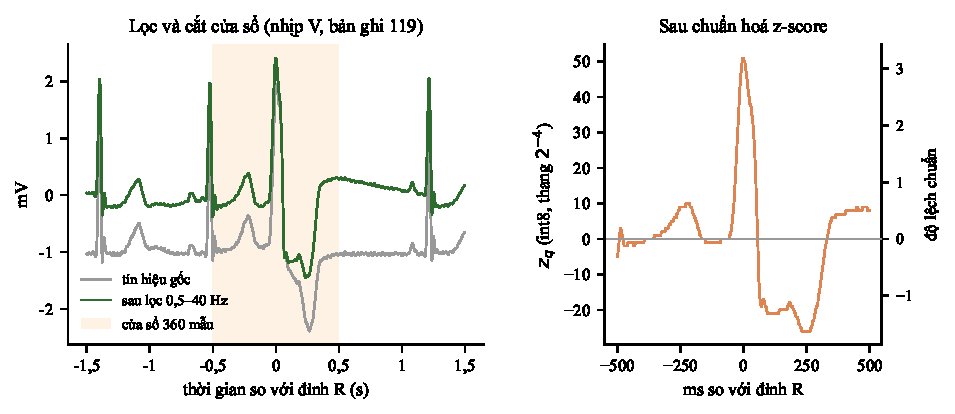
\includegraphics[width=\textwidth]{ch04_mo_hinh_cnn/mot_nhip.pdf}
  \caption{Một nhịp V của bản ghi 119: tín hiệu trước và sau bộ lọc 0{,}5--40\,Hz với vùng cửa sổ 360 mẫu (trái), và cửa sổ sau chuẩn hoá z-score số nguyên (phải).}\label{fig:ch4-motnhip}
\end{figure}

\subsection{Đặc trưng khoảng RR}

Nhịp S chủ yếu khác nhịp N ở thời điểm xuất hiện, thông tin mà cửa sổ một nhịp không có, nên mạng nhận thêm bốn đặc trưng nhịp điệu.
Với $\mathrm{RR}_k=R_k-R_{k-1}$, kẹp trong 0{,}2--3\,s để loại giá trị phi sinh lý:
\begin{equation}
  \mathrm{RR}_{\text{trước}}=\mathrm{RR}_k,\qquad
  \mathrm{RR}_{\text{sau}}=\mathrm{RR}_{k+1},\qquad
  \overline{\mathrm{RR}}=\frac{1}{n}\sum_{j=0}^{n-1}\mathrm{RR}_{k-j},\qquad
  \rho=\frac{\mathrm{RR}_{\text{trước}}}{\overline{\mathrm{RR}}},
  \label{eq:ch4-rr}
\end{equation}
với $n\le8$.
Tỉ số $\rho$ tự chuẩn hoá theo nhịp tim của từng người: nhịp đến sớm có $\rho<1$ dù nhịp tim nhanh hay chậm.
Các đặc trưng chỉ cần thêm một khoảng RR kế tiếp, nên mỗi nhịp chỉ chờ đến đỉnh R sau nó.

\begin{table}[htbp]
  \centering
  \caption{Trung vị của đặc trưng RR theo lớp trên DS1.}\label{tab:ch4-rr}
  \begin{tabular}{lrrrr}
    \toprule
    Đặc trưng & N & S & V & F \\
    \midrule
    $\mathrm{RR}_{\text{trước}}$ (s) & 0{,}756 & 0{,}492 & 0{,}522 & 0{,}592 \\
    $\mathrm{RR}_{\text{sau}}$ (s) & 0{,}736 & 0{,}644 & 0{,}856 & 0{,}461 \\
    $\rho$ & 1{,}00 & 0{,}83 & 0{,}74 & 0{,}96 \\
    \bottomrule
  \end{tabular}
\end{table}

Theo Bảng~\ref{tab:ch4-rr}, nhịp S và V đến sớm ($\rho$ khoảng 0{,}83 và 0{,}74), và nhịp V có khoảng nghỉ bù dài phía sau.
Nhịp F có $\rho$ gần 1, gần như không khác nhịp N về thời điểm, nên chỉ phân biệt được bằng hình dạng; đây là một lý do lớp F khó nhận diện nhất.

Mỗi đặc trưng được lượng tử về int8 với thang $2^{-e_j}$, $e_j=(6,6,6,5)$, bằng một phép chia làm tròn, ví dụ $\mathrm{rr}_{q,0}=\lfloor\mathrm{RR}_{\text{trước}}\cdot2^{6}/360\rceil$; tỉ số được tính thẳng từ tổng các khoảng RR để chỉ chia một lần.
Như vậy khoảng RR có độ phân giải $1/64$\,s, tối đa khoảng 1{,}98\,s, còn tỉ số tối đa khoảng 3{,}97.
